% Compile with Tectonic or XeLaTeX. Run python analysis.py before rebuilding.
\documentclass[a4paper,10pt]{article}
\usepackage[margin=20mm,headheight=14pt,headsep=7mm,footskip=11mm]{geometry}
\usepackage{fontspec}
\setmainfont{texgyreheros-regular.otf}[BoldFont=texgyreheros-bold.otf,ItalicFont=texgyreheros-italic.otf,BoldItalicFont=texgyreheros-bolditalic.otf]
\usepackage[english]{babel}
\usepackage[expansion=false]{microtype}
\usepackage{amsmath,amssymb,siunitx,booktabs,tabularx,array,graphicx}
\usepackage{float,caption,enumitem,fancyhdr,lastpage}
\usepackage{tikz}
\usepackage[american]{circuitikz}
\usetikzlibrary{positioning,arrows.meta,fit,calc,backgrounds}
\usepackage{pgfplots}
\pgfplotsset{compat=1.18}
\usepackage[hidelinks]{hyperref}
\hypersetup{pdftitle={Portable Guitar MultiFX: 5 V Hardware Design and Integration},pdfauthor={Javier Estiven León Calderón},pdfsubject={MFX-AN-001 Revision 0.1; pre-fabrication application note}}
\sisetup{detect-all,round-mode=places,round-precision=3,round-pad=false,group-digits=none}
\setlength{\parindent}{0pt}
\setlength{\parskip}{5pt}
\setlength{\tabcolsep}{4pt}
\renewcommand{\arraystretch}{1.18}
\setlist{nosep,leftmargin=*,topsep=4pt}
\captionsetup{font=small,labelfont=bf,skip=5pt}
\newcolumntype{Y}{>{\raggedright\arraybackslash}X}
\newcolumntype{P}[1]{>{\raggedright\arraybackslash}p{#1}}
\pagestyle{fancy}
\fancyhf{}
\fancyhead[L]{\small\textbf{MultiFX}\quad MFX-AN-001}
\fancyhead[R]{\small Rev. 0.1\quad 26 November 2026}
\fancyfoot[L]{\footnotesize Pre-fabrication design and integration}
\fancyfoot[R]{\footnotesize\thepage\ /\ \pageref{LastPage}}
\renewcommand{\headrulewidth}{0.4pt}
\newcommand{\nextsection}[1]{\clearpage\section{#1}}
\newcommand{\calc}[1]{\num[round-precision=3]{#1}}
\newcommand{\net}[1]{\texttt{#1}}
% Generated by analysis.py; analytical predictions only. Do not edit by hand.
% Units are encoded in macro names or specified in the application note.
\newcommand{\MFXInputResistanceM}{1.006}
\newcommand{\MFXInputResistanceK}{1006}
\newcommand{\MFXInputPoleHz}{0.3350426}
\newcommand{\MFXInputPoleMinHz}{0.3015685}
\newcommand{\MFXInputPoleMaxHz}{0.3760298}
\newcommand{\MFXInputAttenuationDb}{-0.0404857}
\newcommand{\MFXOutputLoadK}{18.37398}
\newcommand{\MFXOutputPoleHz}{8.615085}
\newcommand{\MFXOutputPoleMinHz}{7.82351}
\newcommand{\MFXOutputPoleMaxHz}{9.582731}
\newcommand{\MFXOutputAttenuationDb}{-0.04714459}
\newcommand{\MFXPassbandGainOneDb}{-0.08763029}
\newcommand{\MFXGainTwoMin}{1.904762}
\newcommand{\MFXGainTwoMax}{2.105263}
\newcommand{\MFXVrefPoleHz}{3.183099}
\newcommand{\MFXVrefTauMs}{50}
\newcommand{\MFXVrefRatioMin}{0.475}
\newcommand{\MFXVrefRatioMax}{0.525}
\newcommand{\MFXAnalogPoleHz}{72.34316}
\newcommand{\MFXAnalogPoleMinHz}{57.4152}
\newcommand{\MFXAnalogPoleMaxHz}{95.18836}
\newcommand{\MFXAnalogRailTyp}{4.955224}
\newcommand{\MFXAnalogRailScenario}{4.941294}
\newcommand{\MFXAnalogCurrentTypMilli}{0.4477612}
\newcommand{\MFXAnalogCurrentScenarioMilli}{0.5870647}
\newcommand{\MFXVrefNominal}{2.477612}
\newcommand{\MFXHeadroomMarginV}{0.1}
\newcommand{\MFXConditionerOutputPeak}{2.377612}
\newcommand{\MFXConditionerInputOneRms}{1.68908}
\newcommand{\MFXConditionerInputTwoRms}{0.8445401}
\newcommand{\MFXConditionerInputTwoWorstRms}{0.8023131}
\newcommand{\MFXConditionerDspOutputRms}{1.672125}
\newcommand{\MFXVbusNominal}{3.43985}
\newcommand{\MFXVbusLow}{3.247387}
\newcommand{\MFXVbusHigh}{3.634298}
\newcommand{\MFXAmpGainDb}{23.5}
\newcommand{\MFXAmpGainLinear}{14.96236}
\newcommand{\MFXAmpInputRms}{0.1890362}
\newcommand{\MFXAmpInputRatio}{0.2100402}
\newcommand{\MFXAmpAttenuationDb}{-13.55395}
\newcommand{\MFXLdoPowerFiftyMilli}{85}
\newcommand{\MFXLdoPowerHundredMilli}{170}
\newcommand{\MFXIicRiseNs}{796.462}
\newcommand{\MFXIicCapStandardPf}{251.1105}
\newcommand{\MFXIicCapFastPf}{75.33316}
\newcommand{\MFXResponseTwentyDb}{-0.8280448}
\newcommand{\MFXResponseEightyTwoDb}{-0.1349178}

% Original vector figures. Dimensions are controlled; figure text stays at 9 pt.
\tikzset{mfxbox/.style={draw=black!70,fill=black!3,rounded corners=1pt,align=center,inner sep=4pt,minimum height=9mm},mfxarrow/.style={-{Stealth[length=1.8mm]},line width=.65pt},mfxcontrol/.style={mfxarrow,dashed},mfxlabel/.style={font=\fontsize{9}{10.5}\selectfont,align=center,fill=white,inner sep=2pt},mfxgroup/.style={draw=black!40,rounded corners=2pt,inner sep=5mm}}
\newcommand{\MFXArchitectureDiagram}{%
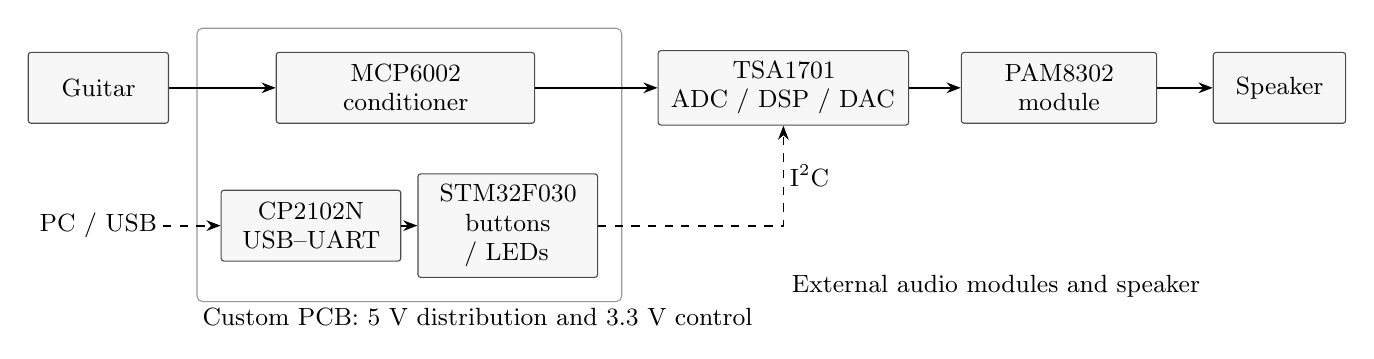
\begin{tikzpicture}[font=\fontsize{9}{10.5}\selectfont,x=1cm,y=1cm]
\node[mfxbox,text width=15mm] (guitar) at (0,0) {Guitar};
\node[mfxbox,text width=30mm] (input) at (3.9,0) {MCP6002\\conditioner};
\node[mfxbox,text width=29mm] (dsp) at (8.7,0) {TSA1701\\ADC / DSP / DAC};
\node[mfxbox,text width=22mm] (amp) at (12.2,0) {PAM8302\\module};
\node[mfxbox,text width=14mm] (speaker) at (15,0) {Speaker};
\node[mfxbox,text width=20mm] (uart) at (2.7,-1.75) {CP2102N\\USB--UART};
\node[mfxbox,text width=20mm] (mcu) at (5.2,-1.75) {STM32F030\\buttons / LEDs};
\node[mfxlabel] (usb) at (0,-1.75) {PC / USB};
\draw[mfxarrow] (guitar)--(input);\draw[mfxarrow] (input)--(dsp);
\draw[mfxarrow] (dsp)--(amp);\draw[mfxarrow] (amp)--(speaker);
\draw[mfxcontrol] (usb)--(uart);\draw[mfxcontrol] (uart)--(mcu);
\draw[mfxcontrol] (mcu.east)--(8.7,-1.75)--node[mfxlabel,right]{I\textsuperscript{2}C}(dsp.south);
\begin{scope}[on background layer]\node[mfxgroup,inner sep=3mm,fit=(input)(uart)(mcu)] (pcb) {};\end{scope}
\node[mfxlabel,anchor=north west] at (pcb.south west) {Custom PCB: 5 V distribution and 3.3 V control};
\node[mfxlabel,anchor=north] at (11.4,-2.3) {External audio modules and speaker};
\end{tikzpicture}}

\newcommand{\MFXInputCircuitDiagram}{%
\begin{circuitikz}[font=\fontsize{9}{10.5}\selectfont]
\node[op amp] (b) at (7.4,0) {U2B};
\draw (.7,0 |- b.+) node[ocirc,label=left:{J2 TIP}]{} to[C,l=C7,a=470 nF] (2.1,0 |- b.+)
 to[R,l=R5,a=4.7 k$\Omega$] (4.3,0 |- b.+) -- (b.+);
\draw (4.9,0 |- b.+) node[circ]{} to[R] (4.9,-2.7);
\node[mfxlabel,anchor=east,align=right] at (4.55,-1.6) {R6 + R7 + R8\\1.006 M$\Omega$};
\node[mfxlabel,anchor=north] at (4.9,-2.8) {VREF\_AUDIO};
\draw (.7,-1.1) node[ocirc,label=left:{J2 SLEEVE}]{} -- (.7,-1.65) node[ground]{};
\draw (b.-) -| (6,1.55) to[R,l=R9,a=10 k$\Omega$] (9.3,1.55) -- (9.3,0) -- (b.out);
\draw (6,1.55) -- (6,2.65) to[nos,l=JP3] (9.3,2.65) -- (9.3,1.55);
\draw (6,1.55) to[R,l_=R10,a^=10 k$\Omega$] (3.5,1.55) node[anchor=east]{VREF\_AUDIO};
\draw (9.3,0) to[R,l=R11,a=100 $\Omega$] (11.2,0) to[C,l=C8,a=1 $\mu$F] (13.3,0) -- (14.5,0) node[ocirc,label=above:{to JP7.1}]{};
\draw (14,0) node[circ]{} to[R,l_=R12,a^=226 k$\Omega$] (14,-2.45) node[ground]{};
\node[mfxlabel] at (8,-1.85) {U2: MCP6002-I/P\\Supply: +5V\_A / GND};
\node[op amp] (a) at (4.4,-4.6) {U2A};
\draw (.5,-3.25) node[anchor=south]{+5V\_A} to[R,l=R3,a=10 k$\Omega$] (.5,-5.09)
 to[R,l=R4,a=10 k$\Omega$] (.5,-6.85) node[ground]{};
\draw (.5,0 |- a.+) node[circ]{} -- (a.+);
\draw (2.1,0 |- a.+) node[circ]{} to[C,l=C6] (2.1,-6.85) node[ground]{};
\draw (a.out) -- (6.7,-4.6) node[ocirc]{} node[anchor=south]{VREF\_AUDIO};
\draw (a.-) -- ++(-.25,0) |- (4,-3.25) -| (5.95,-4.6) node[circ]{};
\node[mfxlabel,align=left,text width=66mm] at (10.8,-5.7) {C6 = 10 $\mu$F filters the divider.\\C5 = 100 nF decouples U2 locally.\\The buffered reference is distinct from system ground.};
\end{circuitikz}}

\newcommand{\MFXResponsePlots}{%
\begin{tikzpicture}
\begin{semilogxaxis}[width=8.25cm,height=6.3cm,xlabel={Frequency (Hz)},ylabel={Source-to-module gain (dB)},xmin=.1,xmax=20000,ymin=-45,ymax=9,grid=both,minor grid style={gray!10},major grid style={gray!25},label style={font=\fontsize{9}{10}\selectfont},tick label style={font=\footnotesize},legend style={font=\footnotesize,at={(.03,.97)},anchor=north west,draw=none,fill=white},legend cell align=left]
\addplot[black,thick] table[x=frequency,y=gain_one_db,col sep=comma]{response.csv};\addlegendentry{JP3 closed: gain 1}
\addplot[gray,thick] table[x=frequency,y=gain_two_db,col sep=comma]{response.csv};\addlegendentry{JP3 open: gain 2}
\addplot[gray,dashed] table[x=frequency,y=gain_two_low_db,col sep=comma]{response.csv};
\addplot[gray,dashed] table[x=frequency,y=gain_two_high_db,col sep=comma]{response.csv};
\end{semilogxaxis}
\begin{axis}[at={(8.45cm,0)},anchor=south west,width=8.1cm,height=6.3cm,xlabel={Analog rail $V_A$ (V)},ylabel={Guitar sine input (V RMS)},xmin=3,xmax=5.25,ymin=0,ymax=2,grid=major,major grid style={gray!25},label style={font=\fontsize{9}{10}\selectfont},tick label style={font=\footnotesize},legend style={font=\footnotesize,at={(.03,.97)},anchor=north west,draw=none},legend cell align=left]
\addplot[black,thick,domain=3:5.25,samples=30]{(x/2-\MFXHeadroomMarginV)/(sqrt(2)*10^(\MFXInputAttenuationDb/20))};\addlegendentry{Nominal gain 1}
\addplot[gray,thick,domain=3:5.25,samples=30]{(x/2-\MFXHeadroomMarginV)/(2*sqrt(2)*10^(\MFXInputAttenuationDb/20))};\addlegendentry{Nominal gain 2}
\node[font=\footnotesize,align=center,anchor=south] at (rel axis cs:.5,.03) {Illustrative reserve: \MFXHeadroomMarginV\ V\\Centered reference; not a swing guarantee};
\end{axis}
\end{tikzpicture}}

\newcommand{\MFXPcbLayoutDiagram}{%
\begin{tikzpicture}[font=\fontsize{9}{10.5}\selectfont]
\node[inner sep=0] (pcbimage) {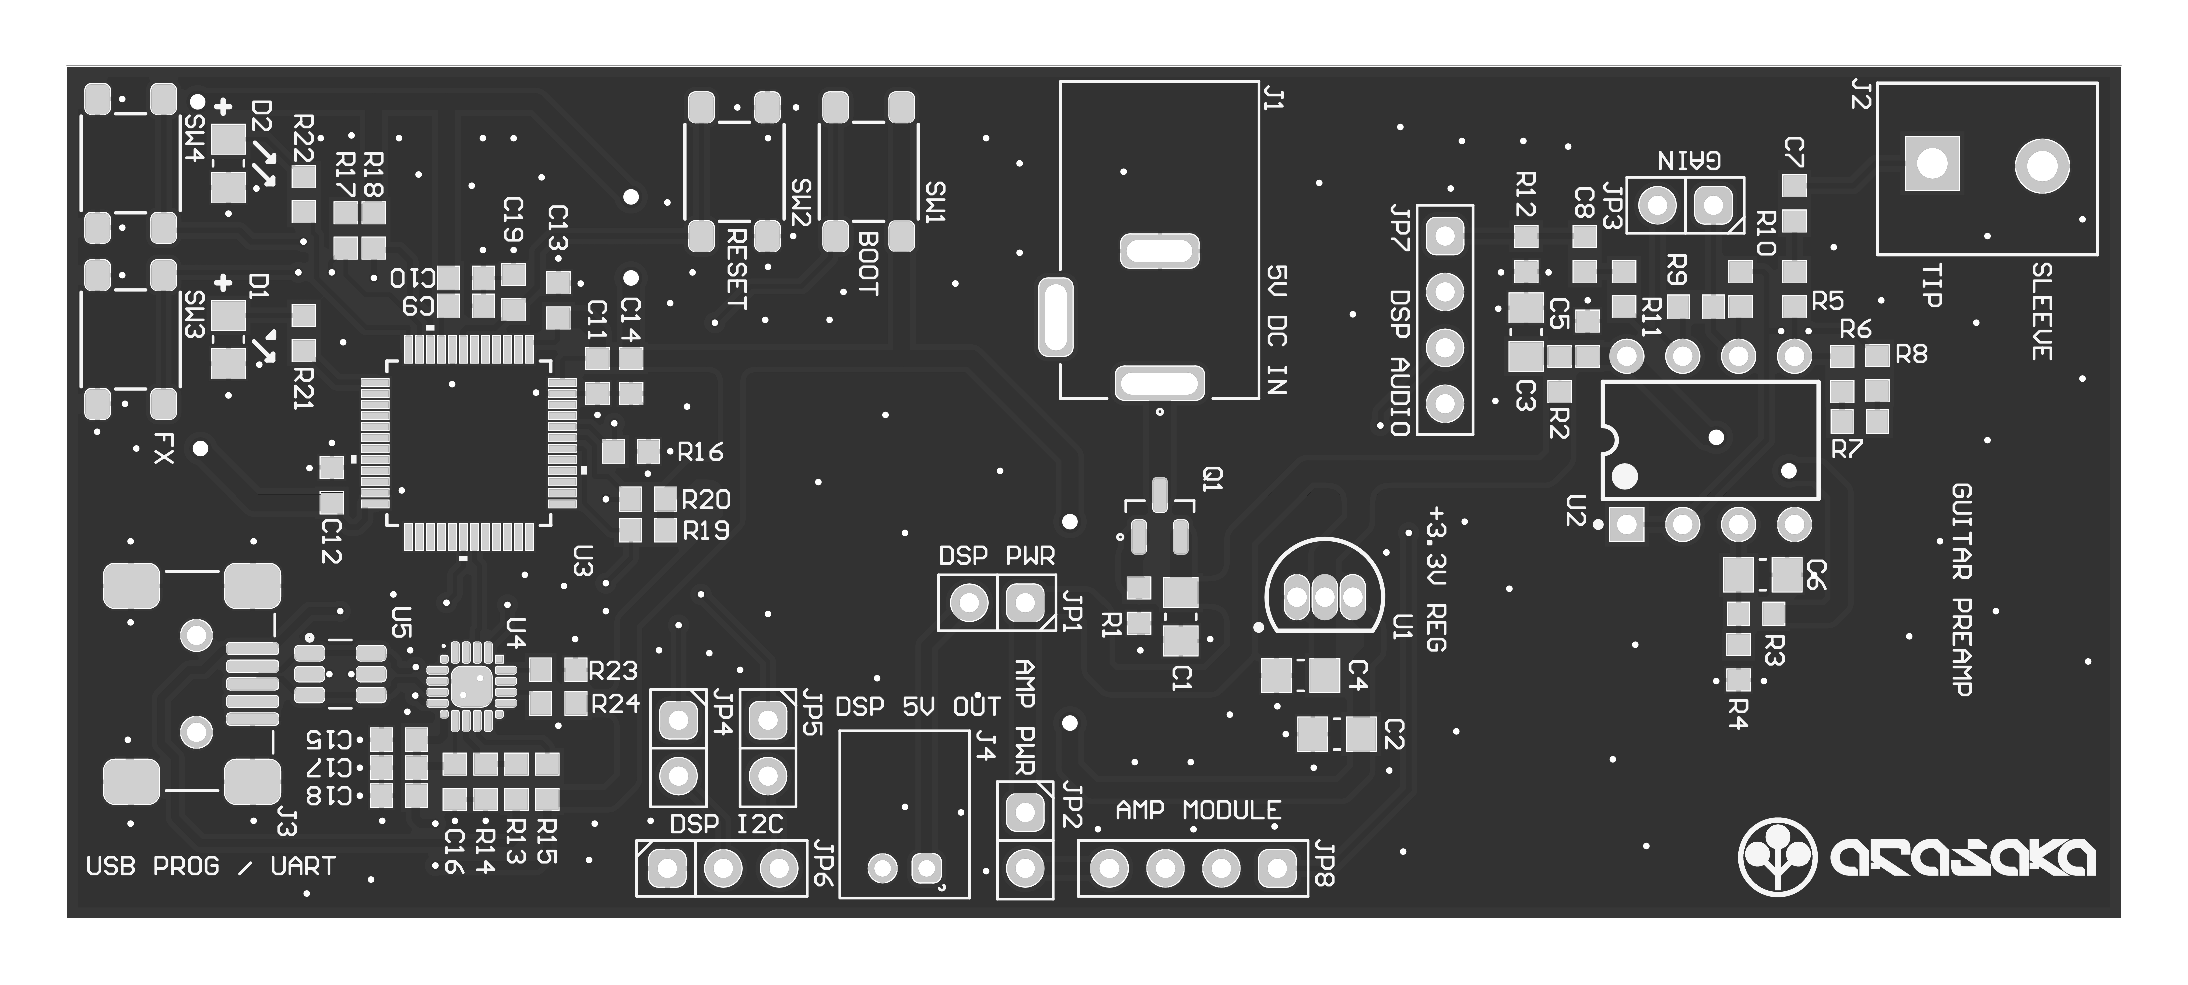
\includegraphics[width=.96\linewidth]{figures/pcb-top.pdf}};
\node[mfxlabel,above=6mm of pcbimage.north west,anchor=south west] (left) {Controller / USB\\Local digital decoupling};
\node[mfxlabel,above=6mm of pcbimage.north] (middle) {5 V entry / regulation\\Supply branches and returns};
\node[mfxlabel,above=6mm of pcbimage.north east,anchor=south east] (right) {Guitar input / U2\\Short, high-impedance path};
\draw[mfxarrow] (left.south)--($(pcbimage.north west)!.22!(pcbimage.north east)+(0,-15mm)$);
\draw[mfxarrow] (middle.south)--($(pcbimage.north west)!.52!(pcbimage.north east)+(0,-20mm)$);
\draw[mfxarrow] (right.south)--($(pcbimage.north west)!.86!(pcbimage.north east)+(0,-10mm)$);
\node[mfxlabel,below=5mm of pcbimage.south] {Inspect both copper layers and cable returns. Regions alone do not prove isolation.};
\end{tikzpicture}}

\newcommand{\MFXConnectionsDiagram}{%
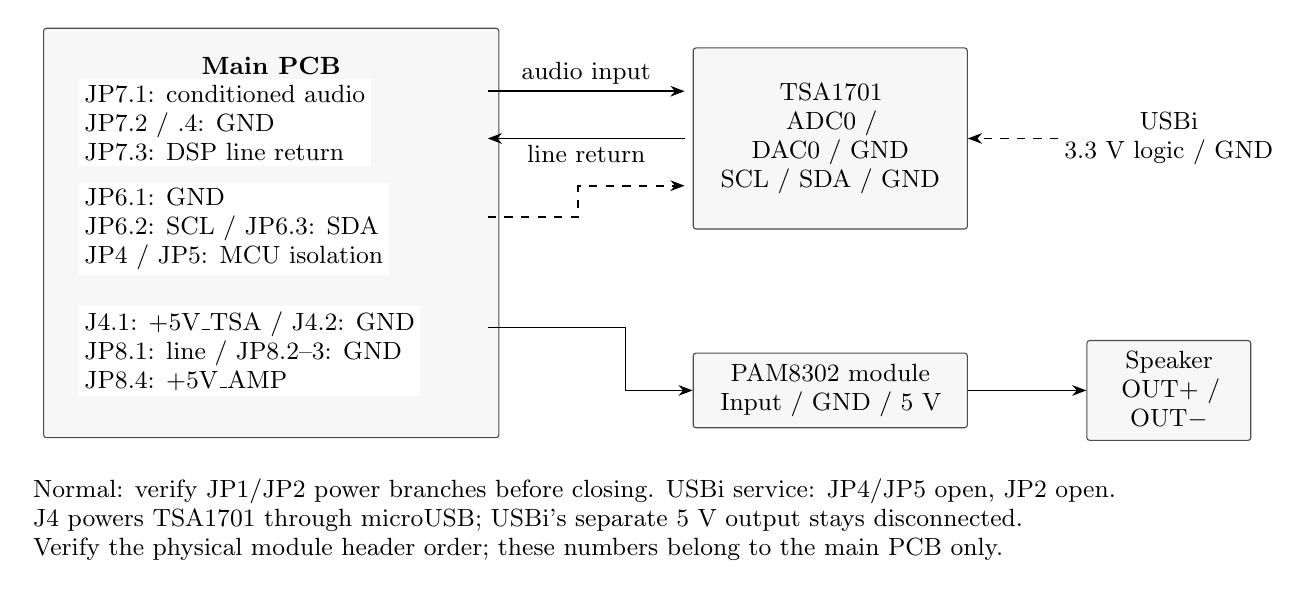
\begin{tikzpicture}[font=\fontsize{9}{10.5}\selectfont,x=1cm,y=1cm]
\node[mfxbox,text width=55mm,minimum height=52mm] (board) at (3.1,0) {};
\node[anchor=north,font=\bfseries\fontsize{9}{10.5}\selectfont] at (3.1,2.35) {Main PCB};
\node[mfxlabel,anchor=west,align=left] at (.65,1.4) {JP7.1: conditioned audio\\JP7.2 / .4: GND\\JP7.3: DSP line return};
\node[mfxlabel,anchor=west,align=left] at (.65,.05) {JP6.1: GND\\JP6.2: SCL / JP6.3: SDA\\JP4 / JP5: MCU isolation};
\node[mfxlabel,anchor=west,align=left] at (.65,-1.5) {J4.1: +5V\_TSA / J4.2: GND\\JP8.1: line / JP8.2--3: GND\\JP8.4: +5V\_AMP};
\node[mfxbox,text width=32mm,minimum height=23mm] (dsp) at (10.2,1.2) {TSA1701\\ADC0 / DAC0 / GND\\SCL / SDA / GND};
\node[mfxbox,text width=32mm] (amp) at (10.2,-2) {PAM8302 module\\Input / GND / 5 V};
\node[mfxbox,text width=18mm] (spk) at (14.5,-2) {Speaker\\OUT+ / OUT$-$};
\node[mfxlabel] (usbi) at (14.5,1.2) {USBi\\3.3 V logic / GND};
\draw[mfxarrow] (5.85,1.8)--node[mfxlabel,above]{audio input}(8.35,1.8);
\draw[mfxarrow] (8.35,1.2)--node[mfxlabel,below]{line return}(5.85,1.2);
\draw[mfxcontrol] (5.85,.2)--(7,.2)--(7,.6)--(8.35,.6);
\draw[mfxcontrol] (usbi.west)--(dsp.east);
\draw[mfxarrow] (5.85,-1.2)--(7.6,-1.2)--(7.6,-2)--(amp.west);
\draw[mfxarrow] (amp.east)--(spk.west);
\node[mfxlabel,align=left,anchor=north west] at (0,-3.05) {Normal: verify JP1/JP2 power branches before closing. USBi service: JP4/JP5 open, JP2 open.\\J4 powers TSA1701 through microUSB; USBi's separate 5 V output stays disconnected.\\Verify the physical module header order; these numbers belong to the main PCB only.};
\end{tikzpicture}}

\newcommand{\MFXTestSetupDiagram}{%
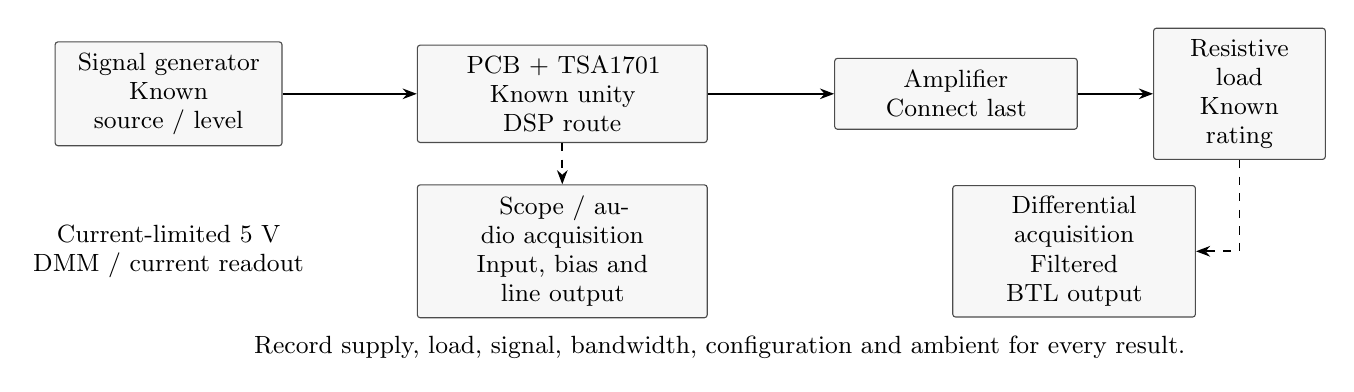
\begin{tikzpicture}[font=\fontsize{9}{10.5}\selectfont,x=1cm,y=1cm]
\node[mfxbox,text width=26mm] (gen) at (1,0) {Signal generator\\Known source / level};
\node[mfxbox,text width=34mm] (dut) at (6,0) {PCB + TSA1701\\Known unity DSP route};
\node[mfxbox,text width=28mm] (amp) at (11,0) {Amplifier\\Connect last};
\node[mfxbox,text width=19mm] (load) at (14.6,0) {Resistive load\\Known rating};
\draw[mfxarrow] (gen)--(dut);\draw[mfxarrow] (dut)--(amp);\draw[mfxarrow] (amp)--(load);
\node[mfxbox,text width=34mm] (scope) at (6,-2) {Scope / audio acquisition\\Input, bias and line output};
\node[mfxbox,text width=28mm] (diff) at (12.5,-2) {Differential acquisition\\Filtered BTL output};
\draw[mfxcontrol] (dut)--(scope);\draw[mfxcontrol] (load.south)|-(diff.east);
\node[mfxlabel] at (1,-2) {Current-limited 5 V\\DMM / current readout};
\node[mfxlabel,anchor=north] at (8,-3) {Record supply, load, signal, bandwidth, configuration and ambient for every result.};
\end{tikzpicture}}

\begin{document}
\thispagestyle{fancy}
{\LARGE\bfseries Portable Guitar MultiFX\par}
{\Large 5 V Hardware Design and Integration\par}
\vspace{2mm}
Javier Estiven León Calderón\quad\textbar\quad Electronic Engineering\par
Universidad Nacional de Colombia

\textbf{Abstract.} A passive electric guitar needs a high-impedance analog interface, while a digital effects module needs controlled signal levels, power, and a separate user-control path. This note explains a custom two-layer PCB combining an MCP6002 conditioner, an STM32F030 controller, and interfaces to external TSA1701 DSP and PAM8302 amplifier modules. It derives the small-signal response, examines gain and supply margins, and specifies connection and verification procedures. The design is documented in CAD; fabrication, assembly, deployed audio/control software, and bench measurements are pending.

\section{Application overview}
\label{sec:overview}
The intended application is a compact mono practice amplifier with physical clean/FX controls and eventual equalization. This revision addresses \emph{hardware design and integration}, not a completed effects algorithm. It is written for an electronics student or engineer reproducing and evaluating the board. The design source is the repository snapshot \net{ad3ab21}~\cite{repo}.

\begin{table}[H]\centering\small
\caption{Design summary and evidence boundary.}\label{tab:spec}
\begin{tabularx}{\linewidth}{P{33mm}P{43mm}Y}\toprule
Parameter & Value or intended behavior & Evidence / condition\\\midrule
Main / control supply & 5 V nominal / 3.3 V nominal & Schematic; usable source range and current budget need closure.\\
Input / gain selection & \SI{\MFXInputResistanceM}{\mega\ohm} bias; gain 1 or 2 & Calculated nominal values; JP3 selects the feedback configuration.\\
Audio / control & TSA1701 / STM32F030C8 & External DSP processes audio; I\textsuperscript{2}C carries parameters.\\
Power stage / load & PAM8302 module; 4 $\Omega$, 5 W speaker & Interface intent. Speaker rating is not amplifier output power.\\
Physical implementation & Five schematic sheets; two-layer PCB & Native Altium files and manufacturing snapshot available.\\
Clean/drive, EQ, performance & Intended software scope & No deployed software or measured system results supplied.\\\bottomrule
\end{tabularx}
\end{table}

\begin{figure}[H]\centering\MFXArchitectureDiagram
\caption{System responsibilities. Solid arrows carry analog audio; dashed arrows carry control or programming data. The main PCB conditions the input and manages interfaces; it does not process audio samples.}\label{fig:architecture}
\end{figure}

\nextsection{Guitar input and reference design}
\label{sec:analog}
A line input alone can load a passive pickup and alter its level and resonance. The conditioner instead presents a high-value bias path, buffers the signal, and removes its local DC bias before the TSA1701 connector. U2 is an MCP6002-I/P; its low-voltage operation and input characteristics support this use, subject to the actual load and output-swing limits~\cite{mcp6002}.

\begin{figure}[H]\centering\MFXInputCircuitDiagram
\caption{Selected signal and reference circuitry, redrawn from schematic sheet 3. R6--R8 are shown as one equivalent element with their actual designators. C5 is local supply decoupling; the drawing is not a replacement for the complete schematic.}\label{fig:input}
\end{figure}

\subsection{Input impedance and bias}
With U2B input current neglected and the buffered reference quiet at AC,
\begin{equation}
R_B=R_6+R_7+R_8=390+390+226=\SI{1006}{\kilo\ohm},\qquad
Z_{\rm in}(s)\simeq R_5+\frac{1}{sC_7}+R_B.
\end{equation}
The approximately 1 M$\Omega$ figure is a midband resistive description, not a complete pickup/cable model. Source resistance, pickup inductance, cable capacitance, protection leakage, and instrument volume settings are excluded from the analytical curves.

R3 and R4 bias U2A, whose output is \net{VREF\_AUDIO}. Ideally,
\begin{equation}
V_{\rm REF}=V_A\frac{R_4}{R_3+R_4}=\frac{V_A}{2},\quad
\tau_{\rm REF}=(R_3\parallel R_4)C_6=\SI{\MFXVrefTauMs}{\milli\second}.
\end{equation}
The unbuffered divider pole is \SI{\MFXVrefPoleHz}{\hertz}. With the BOM's 5\% divider resistors, the divider ratio alone spans 0.475--0.525. It is therefore inappropriate to assume an exact 2.500 V reference. U2A must also source or sink feedback-related signal current in gain-two mode.

Opening JP3 gives $G=1+R_9/R_{10}=2$ around the reference. Closing it bypasses R9 for unity gain. Change this jumper with power removed; it selects analog gain, not the DSP's clean or drive processing mode.

\nextsection{Frequency response and signal margins}
\label{sec:response}
The 5\% R9/R10 tolerances bound gain-two feedback as follows:
\begin{equation}
G_{\min}=1+\frac{0.95R_9}{1.05R_{10}}=\calc{\MFXGainTwoMin},\qquad
G_{\max}=1+\frac{1.05R_9}{0.95R_{10}}=\calc{\MFXGainTwoMax}.
\end{equation}
For an ideal low-impedance source, quiet reference, and ideal op-amps, model the TSA1701 input as its published $R_T=20$ k$\Omega$~\cite{tsa}. With $R_L=R_{12}\parallel R_T$, the loaded response is
\begin{equation}
H(s)=G\frac{sC_7R_B}{1+sC_7(R_5+R_B)}
        \frac{sC_8R_L}{1+sC_8(R_{11}+R_L)}.\label{eq:response}
\end{equation}
The input pole is \SI{\MFXInputPoleHz}{\hertz}; output coupling dominates at \SI{\MFXOutputPoleHz}{\hertz}. R5 and R11 introduce small midband divider losses as well as their other circuit roles. The model predicts gain-one responses of \calc{\MFXResponseTwentyDb} dB at 20 Hz and \calc{\MFXResponseEightyTwoDb} dB at 82.4 Hz, both relative to the source voltage.

\begin{figure}[H]\centering\MFXResponsePlots
\caption{Analytical predictions, not SPICE or measurements. Left: ideal-op-amp response; dashed bounds vary R9/R10 only. Right: illustrative input headroom versus the analog rail with a 0.1 V output reserve, centered reference, and midband passive loss. This reserve is a model parameter, not a guaranteed MCP6002 swing.}\label{fig:response}
\end{figure}

\begin{table}[H]\centering\small
\caption{Selected calculated quantities and their assumptions.}\label{tab:calcs}
\begin{tabularx}{\linewidth}{P{43mm}P{35mm}Y}\toprule
Quantity & Result & Conditions / limits\\\midrule
Input coupling pole & 0.302--0.376 Hz & Initial R5, R6--R8 and C7 tolerances.\\
Output coupling pole & 7.824--9.583 Hz & Initial R11, R12 and C8 tolerances; $R_T$ fixed at 20 k$\Omega$.\\
Gain-one midband loss & \calc{\MFXPassbandGainOneDb} dB & Both passive dividers; no pickup loading model.\\
Analog RC pole & \calc{\MFXAnalogPoleHz} Hz & 100 $\Omega$ and 22 $\mu$F nominal; small-signal, lightly loaded case.\\
Headroom example, gain 1 / 2 & \calc{\MFXConditionerInputOneRms} / \calc{\MFXConditionerInputTwoRms} V RMS & Sinusoid, nominal bias, estimated $V_A$, 0.1 V reserve; not a clipping specification.\\\bottomrule
\end{tabularx}
\end{table}

\subsection{Keep distortion in the intended stage}
The 5 V rail cannot provide an arbitrary signal excursion. For a general reference and a selected reserve $V_m$, the op-amp's modelled peak allowance is
\begin{equation}
V_{o,\rm pk}\le\min(V_{\rm REF}-V_m,\;V_A-V_{\rm REF}-V_m).
\end{equation}
Reference tolerance, loading, temperature, and finite bandwidth reduce confidence in a nominal estimate. Validate clipping with the actual guitar and DSP input before increasing gain. Intentional drive in a later DSP program cannot recover peaks already clipped by the analog stage or ADC. The TSA1701's published 2 V RMS input range does not require this conditioner to deliver 2 V RMS.

\nextsection{Power distribution and interface limits}
\label{sec:power}
J1 supplies \net{VIN\_5V\_RAW}; Q1 is the P-channel reverse-polarity arrangement shown in the source. The BOM identifies an ALLPOWER AP2301: confirm that exact device's pinout and ratings rather than borrowing another vendor's similarly named part. JP1 connects the DSP branch and JP2 the amplifier branch. R2/C3 isolate the sensitive analog rail; U1 is the MCP1700-3302E/TO for the control rail~\cite{mcp1700}.

\subsection{Budget by branch, then select the source}
\begin{table}[H]\centering\small
\caption{Power budget to complete at bring-up. Entries are not measured demands.}\label{tab:power}
\begin{tabularx}{\linewidth}{P{29mm}P{47mm}Y}\toprule
Branch & Analytical basis & Required closure\\\midrule
Analog conditioner & $I_A\simeq2I_Q+V_A/(R_3+R_4)$ & Supply current plus actual signal/reference loading.\\
3.3 V control & STM32, CP2102N, LEDs and pull-ups & Clock/activity states, enumeration, GPIO currents and startup.\\
TSA1701 & Entire board, not just ADAU1701 & Standalone boot, program and potentiometer loading.\\
PAM8302 / speaker & $I\simeq P_o/(\eta V_{\rm AMP})+I_{\rm idle}$ & Module efficiency, waveform, distortion and transient demand.\\
Main input & Sum of branch demands and losses & Source tolerance, cable/jack drop, startup, headroom and temperature.\\\bottomrule
\end{tabularx}
\end{table}

An unloaded-reference estimate using $I_Q=100$ $\mu$A per amplifier and a post-Q1 5 V rail gives
\begin{equation}
V_A=\frac{5-2R_2I_Q}{1+R_2/(R_3+R_4)}=\SI{\MFXAnalogRailTyp}{\volt},\quad
I_A=\SI{\MFXAnalogCurrentTypMilli}{\milli\ampere}.
\end{equation}
The MCP6002 data quote that current at different bias/supply test conditions; it is used here as a scenario, not a guaranteed 5 V operating current~\cite{mcp6002}. Substituting 170 $\mu$A per channel gives \calc{\MFXAnalogRailScenario} V under the same simplified assumptions. Reference-output current, dynamic loading and Q1 drop are excluded. The nominal R2/C3 pole spans about 57.4--95.2 Hz with initial component tolerances; effective MLCC capacitance can shift it further.

For the LDO, $P_D\simeq(V_{\rm SYS}-3.3)I_{3.3}$. At 5 V, illustrative 50/100 mA loads dissipate 85/170 mW, excluding ground current. The datasheet's TO-92 thermal characterization uses a stated test board; it is not the temperature rise of this two-layer PCB. Check capacitor stability requirements, effective capacitance, dropout and junction-temperature margin at the actual load.

\subsection{USB sensing is not USB power}
J3 VBUS feeds the CP2102N sense divider and ESD reference; it does not feed \net{+5V\_SYS}. U4 VDD and VREGIN use the external 3.3 V rail. The main supply is required for UART enumeration. The R13/R14 divider gives \calc{\MFXVbusNominal} V at 5 V; an illustrative 4.75--5.25 V source with 1\% resistors gives \calc{\MFXVbusLow}--\calc{\MFXVbusHigh} V. At a nominal 3.3 V I/O supply, these values exceed the 2.7 V detection threshold and remain below the 5.8 V absolute limit~\cite{cp2102n}. This does not establish USB compliance. Silicon Labs also describes divider current limiting when unpowered; verify that case and the actual rail tolerance instead of treating VBUS as an ordinary 3.3 V GPIO.

\nextsection{Controller, programming and DSP ownership}
\label{sec:control}
The STM32F030C8T6TR reads the buttons and drives indicators. CP2102N TXD connects to STM32 PA10/RX; STM32 PA9/TX connects to CP2102N RXD. PB6/PB7 provide SCL/SDA through JP4/JP5. The intended responsibilities require firmware; no implementation or compiled image was supplied~\cite{stm32}.

\begin{table}[H]\centering\small
\caption{Board-side interfaces verified against schematic pin numbers.}\label{tab:interfaces}
\begin{tabularx}{\linewidth}{P{24mm}P{76mm}Y}\toprule
Interface & Pins or connection & Use\\\midrule
J2 & 1: guitar TIP; 2: SLEEVE/GND & Instrument input.\\
J4 & 1: +5V\_TSA; 2: GND & Power cable to TSA1701 microUSB.\\
JP6 & 1: GND; 2: DSP\_SCL; 3: DSP\_SDA & Module control, 3.3 V logic.\\
JP7 & 1: GTR\_TO\_DSP; 2: GND; 3: DSP\_LINE\_OUT; 4: GND & Conditioned ADC0 input and DAC0 return.\\
JP8 & 1: DSP\_LINE\_OUT; 2: GND; 3: GND; 4: +5V\_AMP & PAM8302 input and supply.\\
JP1 / JP2 & 1: +5V\_SYS; 2: +5V\_TSA / +5V\_AMP & Power-branch isolation.\\
JP4 / JP5 & 1: MCU side; 2: DSP side & SCL / SDA service isolation.\\
JP3 & Closed: gain 1; open: gain 2 & Analog feedback only.\\\bottomrule
\end{tabularx}
\end{table}

This table describes \emph{our board}, not a guaranteed order on a commercial module header. Check each module's orientation, ground continuity and documentation before making a cable. A matching connector size does not establish pin compatibility.

\subsection{Manual UART boot procedure}
For STM32F030x8, ST documents system-memory USART1 on PA9/PA10, an internal clock, and boot selection with BOOT0 high and nBOOT1 set to 1~\cite{an2606}. With a verified supply and suitable PC driver, hold BOOT (SW1), press and release RESET (SW2), then release BOOT after reset sampling. Use a compatible USART bootloader tool with even parity (8E1), no hardware flow control, and the prescribed synchronization/ACK exchange~\cite{an3155}. Identify the device before programming. With BOOT released, reset again for Flash execution. This is a proposed procedure; enumeration, option bits and programming have not been demonstrated. No dedicated SWD header is identified in the supplied schematic.

\subsection{Share the bus deliberately}
R19/R20 provide 4.7 k$\Omega$ pull-ups on the MCU side. Opening JP4/JP5 isolates these as well as the MCU; verify pull-ups on the DSP/programmer side. The ADAU1701 owns I\textsuperscript{2}C as master during EEPROM self-boot, then accepts external control~\cite{adau,an923}. Firmware must defer transactions, use bounded timeouts, and export parameter addresses/encoding from the actual SigmaStudio build. In self-boot, the 8-bit address bytes 0x68/0x69 correspond to 7-bit 0x34. Check the MCU API convention and actual configuration.

For one 4.7 k$\Omega$ pull-up and an assumed 200 pF bus, $t_r\simeq0.8473R_PC_B=\SI{\MFXIicRiseNs}{\nano\second}$. This illustrates why 400 kHz cannot be assumed: a 300 ns limit would permit only about \calc{\MFXIicCapFastPf} pF~\cite{i2c}. Start conservatively and measure the complete bus, including parallel pull-ups and unpowered states.

\nextsection{PCB implementation and manufacturing snapshot}
\label{sec:pcb}
The source contains five hierarchical sheets and a two-layer PCB. Its narrow outline places the guitar input and conditioner at one end, the power circuitry near the center, and the controller/USB interface at the other end. The following view makes these functional regions visible without implying that a board has been fabricated.

\begin{figure}[H]\centering\MFXPcbLayoutDiagram
\caption{Top-side view rendered from the supplied Gerber/drill snapshot, with functional annotations. Colors are illustrative. The source SVG records hashes of the rendered layers; this is not an assembly photograph, a DRC result, or proof that the export matches the latest editable PCB.}\label{fig:pcb}
\end{figure}

\subsection{Layout reasoning and checks}
Keep the high-impedance guitar node short and away from USB, clocks, class-D outputs and their return currents. Locate the bias buffer and analog decoupling near U2. Return high speaker/power currents toward their source rather than through input-reference paths. Inspect copper continuity and actual current loops on both layers; colored regions alone do not prove electrical isolation or good grounding.

Place supply capacitors close to their pins, preserving short return loops. Keep USB data routing and ESD placement consistent with the transceiver guidance. Check jack and header polarity, mounting clearances, package orientation and cable exit space against the actual parts and STEP model. The amplifier is external, but its wiring can still inject switching noise into this board.

\subsection{What the supplied manufacturing files establish}
The Gerber ZIP contains 20 files: copper, masks, silkscreen, paste, mechanical plots, round/slotted plated drill data and reports. Its entries match the corresponding raw project outputs byte for byte. The .GM profile and additional .GM2 drawing are different plots; confirm the intended outline with the fabricator rather than treating them as interchangeable.

The generation report is dated 15 November 2026 at 14:47, before the authoritative PCB file's later last-write time. A timestamp difference alone does not prove an electrical change, but equivalence remains unestablished. The older PCB copies in the delivery archives also differ from the authoritative source. Before ordering, freeze the chosen PCB revision, run the appropriate ERC/DRC, regenerate or reconcile its outputs, and inspect layer/drill mapping. This application note does not release that package for manufacturing.

\nextsection{Module connections and staged bring-up}
\label{sec:bringup}
\begin{figure}[H]\centering\MFXConnectionsDiagram
\caption{Connection intent using verified board pin numbers. Module-side physical pin order is deliberately unspecified. During USBi service, open JP4/JP5, keep the amplifier disconnected, and use one documented power arrangement.}\label{fig:connections}
\end{figure}

\subsection{Before power}
Inspect soldering, polarity and shorts on the assembled board. Verify U1/U2 footprints against their actual TO-92/PDIP parts, not merely their library names. Connect the guitar jack sleeve to ground. Leave JP1/JP2 and JP4/JP5 open for the first bare-board checks; set JP3 closed for unity gain. Disconnect the speaker and external modules. Start from a current-limited 5 V source, with the limit chosen from the assembled bare-board load and supply/device constraints.

\begin{enumerate}
\item \textbf{Check the board rails.} Power J1; verify input polarity, +5V\_SYS, +3V3\_CTRL and +5V\_A. Record input current and inspect for unexpected heating. Stop on a rail outside the applicable part limits or an unexplained current excess.
\item \textbf{Check the analog DC operating point.} Measure the divider, VREF\_AUDIO and U2B output, allowing the reference and coupling capacitors to settle. Compare with measured $V_A$ and tolerance predictions, not an assumed exact 2.5 V.
\item \textbf{Verify USB/UART.} With main power present, connect J3 and check enumeration and the BOOT/reset procedure. Check powered/unpowered USB behavior before routine cable changes.
\item \textbf{Add the DSP without the amplifier.} Remove power, verify the TSA1701 cable, close JP1 and power the module through J4/microUSB. Program a known unity audio route with USBi using its documented logic interface and common ground. Leave USBi's separate 5 V output disconnected; do not parallel power outputs.
\item \textbf{Establish standalone and external control.} Check EEPROM boot and quiet line output without the PC. Close JP4/JP5 only after MCU firmware defers bus activity appropriately. Demonstrate one controlled parameter change before enabling the power stage.
\item \textbf{Add the amplifier last.} Remove power; verify JP8 wiring and module input sensitivity. Close JP2 only after gain/startup checks. Connect the selected speaker between OUT+ and OUT$-$ on the amplifier module, never to board ground.
\end{enumerate}

There is no amplifier shutdown/mute control in JP8. Opening JP2 or disconnecting the amplifier is the available staged-isolation method. Safe startup audio therefore depends on verified DSP behavior and the actual module; do not assume firmware can assert a hardware mute that is not wired.

\nextsection{Verification method and gain budgeting}
\label{sec:verification}
\subsection{Reproduce the predictions}
The accompanying \net{analysis.py} uses only Python's standard library. It checks source hashes, computes the linear transfer function and tolerance corners, and generates the values and CSV read by this document. Internal checks include independent KCL forms, DC rejection, high-frequency divider limits, a two-pole low-frequency slope, gain scaling, and finite positive operating quantities. These checks establish agreement with the stated model, not with a physical board.

The curve assumes an ideal source, quiet reference and ideal op-amps. It omits pickup/cable interaction, finite gain-bandwidth, slew rate, noise, distortion, capacitor bias/temperature/aging and unknown module networks. The gain-two envelope varies R9/R10 only; the pole intervals in Table~\ref{tab:calcs} are separate initial-tolerance calculations. Do not interpret either as an exhaustive system tolerance bound.

\subsection{Match DAC level to amplifier sensitivity}
TinySine publishes a 0.9 V RMS TSA1701 output~\cite{tsa}. As a conditional example, the PAM8302A IC data give 23.5 dB gain and about 2 W typical at 5 V, 4 $\Omega$, 1 kHz and 1\% THD+N~\cite{pam}. Thus,
\begin{equation}
A_v=10^{23.5/20}=\calc{\MFXAmpGainLinear},\quad
V_{i,\rm rms}=\frac{\sqrt{2\cdot4}}{A_v}=\SI{\MFXAmpInputRms}{\volt}.
\end{equation}
That example requires a level ratio of about \calc{\MFXAmpInputRatio} (\calc{\MFXAmpAttenuationDb} dB) from a 0.9 V RMS source. The commercial module may include a potentiometer or input network; identify it before selecting attenuation. Neither the full DAC level nor the speaker's 5 W rating establishes clean output power. A digital level reduction may be suitable after the actual DSP startup and module gain are known; it is not implemented evidence in this handoff.

\begin{figure}[H]\centering\MFXTestSetupDiagram
\caption{Proposed staged verification setup. Start with line-level tests and amplifier isolation. When testing class-D power output, use an appropriate differential/isolated measurement method and filtering; a grounded probe clip must not short an active BTL output.}\label{fig:test}
\end{figure}

For every future result record source revision, firmware/DSP versions, jumper state, supply at the board, load, stimulus frequency/amplitude, instrument bandwidth and uncertainty, and ambient/settling conditions. Plot an analytical prediction beside the corresponding measurement only when those conditions support the comparison.

\nextsection{Validation protocol and interpretation}
\label{sec:tests}
\begin{table}[H]\centering\small
\caption{Planned tests. All rows remain pending; no readings are implied.}\label{tab:tests}
\begin{tabularx}{\linewidth}{P{16mm}P{45mm}Y}\toprule
Test & Setup / observable & Evaluation basis\\\midrule
T1 Rails & Bare PCB, modules isolated; DMM and input-current readout. & Check polarity, operating limits, source drop and unexplained load against the branch budget.\\
T2 Bias & Measure $V_A$, divider, reference and U2B DC output after settling. & Compare ratio and load drop with actual resistor values; investigate asymmetry before audio.\\
T3 Analog & Begin at 50 mV RMS, 1 kHz, verified at J2; sweep 20 Hz--20 kHz in both JP3 states, amplifier isolated. & Declare generator impedance/load setting. Compare with Eq.~\ref{eq:response} and uncertainty; increase level gradually to identify clipping.\\
T4 DSP & Known unity program, USBi removed, repeated power/reset cycles; scope line output and inspect I\textsuperscript{2}C. & Confirm autonomous boot, bus handover, one parameter change and bounded error recovery; retain the exact program/map.\\
T5 UART / USB & Main power plus J3, then each documented powered/unpowered transition. & Enumerate, identify/program STM32 through the supported boot pattern; check sense thresholds and injection guidance.\\
T6 Power audio & Verified amplifier gain, specified resistive load, differential acquisition and suitable analysis filter. & Report power \emph{at a stated distortion}, supply and frequency. Verify startup transients and compare to the actual module's documented conditions.\\
T7 Thermal & Declared waveform/load, enclosure state and ambient; temperature/current logging to steady behavior. & Verify part junction/ambient margins with an appropriate model; report temperature locations and uncertainty.\\\bottomrule
\end{tabularx}
\end{table}

The small initial stimulus in T3 is a commissioning step, not a declared guitar-input rating. Define the eventual supported guitar range from measured peaks and the verified margin in both gain modes. Likewise, a frequency-response target, noise/SNR, latency and output-power requirement must be agreed and then tested; none can be inferred from CAD existence alone.

\subsection{Use discrepancies to locate the fault}
\begin{itemize}
\item A gain or bias error with the DSP disconnected first points to JP3, resistor values, reference loading, wiring or op-amp operation. Confirm the generator and scope loading before changing the circuit.
\item A low-frequency difference may be caused by effective coupling capacitance, module input impedance or the test fixture. Measure these conditions before rejecting the two-pole model.
\item Audio clicks at startup or failed parameter changes require checking DSP boot, bus ownership and power sequencing. A parameter address from another SigmaStudio compilation is not a valid substitute.
\item Noise that appears only with the amplifier connected suggests examining shared supply/return impedance, cable placement and class-D measurement technique. A broad-band oscilloscope trace alone is not an audio-noise measurement.
\end{itemize}

\subsection{Evidence needed to close this revision's limits}
Record a reconciled assembly BOM and an identified source revision first. Then retain ERC/DRC and output-review results, module identities, programming records, and measured tables/plots. A subsequent revision may replace the pending entries with evidence; it must preserve test conditions and explain any design change rather than rewriting predictions as successful measurements.

\nextsection{Design resources, reproducibility and limits}
\label{sec:resources}
\subsection{Source package}
The public repository provides editable Altium source, five-page schematic PDF, BOM spreadsheet, native Draftsman document, STEP model, and Gerber/drill snapshot~\cite{repo}. The source project and Draftsman folder are kept as siblings so their relative reference remains valid. Earlier delivery copies and original archives are preserved separately. Use the authoritative project for continued editing, not an arbitrary archived PCB.

\begin{enumerate}
\item Read the current hardware guide and source-revision notes.
\item Run \net{python analysis.py --check} in this note's folder. If deliberately updating the design, review the model and source hashes before regenerating its three data files with \net{python analysis.py}.
\item Compile \net{application-note.tex} using Tectonic or XeLaTeX; retain \net{derived-values.tex}, \net{response.csv}, \net{figures/diagrams.tex} and \net{figures/pcb-top.pdf} beside it. In Overleaf, select this file as the main document and use XeLaTeX.
\item Review the resulting PDF at normal reading size, including every graph, reference and connector label. Compilation alone does not validate a diagram or circuit.
\end{enumerate}

\subsection{Open items in the delivered design}
The BOM export has 27 groups and 59 listed parts but omits JP1--JP8; U1/U2 manufacturer/ordering fields are blank although the schematic identifies their parts. Reconcile fitted headers, jumper shunts, connectors, external modules and mechanical hardware before purchasing. Do not derive an assembly-complete parts list from that export alone.

Standalone component libraries were not supplied: placed objects reference \net{shared\_lib.IntLib} and Altium Content Vault. Restore the required sources before library-driven updates. The original OutJob retains absolute export destinations from the earlier folder layout; select the current destination before generating outputs. Two CAM sessions and a referenced DRC HTML report are absent. No clean-rule-check conclusion is available from those references.

The physical TSA1701 and PAM8302 revisions, module pull-ups and input network, actual supply/cable limits, final enclosure and complete power budget remain to establish. Software delivery must include the STM32 source/build information and the deployed SigmaStudio program with its parameter map. A conceptual enclosure illustration is not hardware evidence.

\subsection{Document basis and revision}
This note adopts the focused problem--mechanism--evidence approach of TI's SLOA238A and the reproducible connection/board-documentation approach of SLOU457~\cite{example-report,example-guide}. The professor's power-design examples similarly motivate the requirement--calculation--implementation--verification chain. Their device ratings, measurements and automotive/motor requirements are not transferred to MultiFX.

Revision 0.1 establishes a reproducible pre-fabrication analysis and operating procedure for source \net{ad3ab21}. It does not introduce changes to the supplied circuit or PCB. Fabrication, assembly and measured verification are the next evidence-producing steps.

\clearpage
\section*{References}
\addcontentsline{toc}{section}{References}
\begingroup\small
\renewcommand{\refname}{}
\vspace{-7mm}
\begin{thebibliography}{99}
\bibitem{repo} J. E. León Calderón, \emph{Portable Guitar MultiFX}, source snapshot \net{ad3ab21}, 26 Nov. 2026. \href{https://github.com/SlLeonn/MultiFx_Project/tree/ad3ab214415b7b048fcca606c6cc5987dbe40415}{Repository and design resources}.
\bibitem{mcp6002} Microchip, \emph{MCP6001/1R/1U/2/4, 1 MHz low-power op amps}, DS20001733L, 2020, electrical characteristics and application guidance. \href{https://ww1.microchip.com/downloads/aemDocuments/documents/MSLD/ProductDocuments/DataSheets/MCP6001-1R-1U-2-4-1-MHz-Low-Power-Op-Amp-DS20001733L.pdf}{Manufacturer datasheet}.
\bibitem{tsa} TinySine, \emph{TSA1701 Audio DSP Board}, module interfaces and published levels, consulted 26 Nov. 2026. \href{https://www.tinysineaudio.com/products/tsa1701-audio-dsp-board}{Module documentation}. Physical revision and operating conditions remain to confirm.
\bibitem{mcp1700} Microchip, \emph{MCP1700 low-quiescent-current LDO}, DS20001826F, 2020, stability, dissipation and package conditions. \href{https://ww1.microchip.com/downloads/aemDocuments/documents/APID/ProductDocuments/DataSheets/MCP1700-Data-Sheet-20001826F.pdf}{Manufacturer datasheet}.
\bibitem{cp2102n} Silicon Labs, \emph{CP2102N USBXpress Family}, Rev. 1.5, external-regulator configuration and VBUS requirements, sections 2.3, 3.1.7 and 3.3. \href{https://www.silabs.com/documents/public/data-sheets/cp2102n-datasheet.pdf}{Manufacturer datasheet}.
\bibitem{stm32} STMicroelectronics, \emph{STM32F030x4/x6/x8/xC}, DS9773 Rev. 5, Nov. 2021. \href{https://www.st.com/resource/en/datasheet/stm32f030c8.pdf}{Manufacturer datasheet}.
\bibitem{an2606} STMicroelectronics, \emph{STM32 microcontroller system memory boot mode}, AN2606 Rev. 71, STM32F030x8 configuration, section 15.1 and boot-pattern table. \href{https://www.st.com/resource/en/application_note/an2606-introduction-to-system-memory-boot-mode-stmicroelectronics.pdf}{Application note}.
\bibitem{an3155} STMicroelectronics, \emph{USART protocol used in the STM32 bootloader}, AN3155 Rev. 21, synchronization and parity. \href{https://www.st.com/resource/en/application_note/an3155-how-to-use-usart-protocol-in-bootloader-on-stm32-mcus-stmicroelectronics.pdf}{Application note}.
\bibitem{adau} Analog Devices, \emph{ADAU1701 SigmaDSP processor}, Rev. C, 2016, control port, self-boot and safeload. \href{https://www.analog.com/media/en/technical-documentation/data-sheets/ADAU1701.pdf}{Manufacturer datasheet}.
\bibitem{an923} J. Lewis, Analog Devices, \emph{Designing a System Using the ADAU1701/ADAU1702 in Self-Boot Mode}, AN-923. \href{https://www.analog.com/en/resources/app-notes/an-923.html}{Application note}.
\bibitem{i2c} Texas Instruments, \emph{I\textsuperscript{2}C Bus Pullup Resistor Calculation}, SLVA689A, rise-time and sink-current constraints. \href{https://www.ti.com/lit/pdf/slva689}{Application note}.
\bibitem{pam} Diodes Incorporated, \emph{PAM8302A 2.5 W filterless mono class-D audio amplifier}, DS41333 Rev. 6-2, May 2021, pp. 3 and 7. \href{https://www.diodes.com/datasheet/download/PAM8302A.pdf}{Manufacturer datasheet}. IC-level example; commercial module implementation must be identified.
\bibitem{example-report} P. Cao, Texas Instruments, \emph{Achieve Ultra-Low Idle Current With TPA3128D2, TPA3156D2, or TPA3126}, SLOA238A, May 2018. \href{https://www.ti.com/lit/pdf/sloa238}{Application report}; supplied as a structural example, not a MultiFX component specification.
\bibitem{example-guide} Texas Instruments, \emph{TPA3128D2 Evaluation Module}, SLOU457, Dec. 2016. \href{https://www.ti.com/lit/pdf/slou457}{User's guide}; supplied as a connection and board-documentation example.
\end{thebibliography}
\endgroup
\end{document}
